% bayes-theorem.tex
\documentclass[12pt,letterpaper]{letter}
\usepackage{fullpage,color,graphicx}
\usepackage[procnames]{listings}
\pagenumbering{gobble}

\newcommand{\assignment}{Bayes Theorem}
\newcommand{\myinfo}
{Darin Critchlow
\\CSIS 2430-001}
\newcommand{\assignmentDescription}
{You will be implementing a Generalized Bayes Theorem (pg 472).  It should handle French guy\textbackslash{Financial vids}.}
\newcommand{\worked}
{Everything worked properly}
\newcommand{\didntwork}
{Everything worked properly}
\newcommand{\comments}
{It was interesting implementing the general form and working out how to loop through the data based upon the name given.
}

\begin{document}

\LARGE\textbf{\assignment{}}

\normalsize\myinfo{}

\textbf{\underline{Objective:}}

\textbf{\assignmentDescription{}}

\textbf{\underline{What Worked:}}

\worked{}

\textbf{\underline{What Didn't Work:}}

\didntwork{}

%\pagebreak
\textbf{\underline{Comments:}}

\comments{}

\pagebreak
\definecolor{keywords}{RGB}{255,127,0}
\definecolor{comments}{RGB}{169,169,169}
\definecolor{red}{RGB}{160,0,0}
\definecolor{green}{RGB}{46,139,87}

\lstset{language=Python,
        basicstyle=\ttfamily\small,
        keywordstyle=\color{keywords},
        commentstyle=\color{comments},
        stringstyle=\color{green},
        showstringspaces=false,
        identifierstyle=\color{black},
        procnamekeys={def,class}}
\textbf{\underline{Code:}}
\lstinputlisting[language=Python]{bayes-theorem.py}

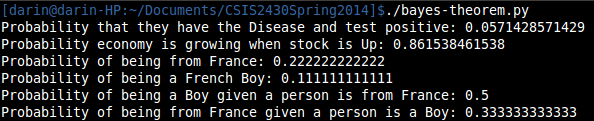
\includegraphics[width=470pt]{bayes_theorem}
\end{document}
